% %                                                                 aa.dem
% % AA vers. 9.1, LaTeX class for Astronomy & Astrophysics
% % demonstration file
%                                                       (c) EDP Sciences
%-----------------------------------------------------------------------
%
% \documentclass[referee]{aa} % for a referee version
%\documentclass[onecolumn]{aa} % for a paper on 1 column  
%\documentclass[longauth]{aa} % for the long lists of affiliations 
%\documentclass[letter]{aa} % for the letters 
%\documentclass[bibyear]{aa} % if the references are not structured 
%                              according to the author-year natbib style

\documentclass[article]{aa}  

%
\usepackage{graphicx}
\usepackage{amsmath,amsfonts,amssymb}
\usepackage{natbib}

%%%%%%%%%%%%%%%%%%%%%%%%%%%%%%%%%%%%%%%%
\usepackage{txfonts}
\usepackage{xcolor}

\usepackage{blindtext}
\usepackage{siunitx}
\DeclareSIUnit\arcmin{arcmin}
%%%%%%%%%%%%%%%%%%%%%%%%%%%%%%%%%%%%%%%%
% \usepackage[options]{hyperref}
% To add links in your PDF file, use the package "hyperref"
% with options according to your LaTeX or PDFLaTeX drivers.
\usepackage{float}
%\usepackage{stfloats}
\usepackage{dblfloatfix}
\usepackage{afterpage}
\usepackage{ifthen}
\usepackage[morefloats=12]{morefloats}

\usepackage{placeins}
\usepackage{multicol}
%\usepackage[breaklinks,colorlinks,citecolor=blue]{hyperref}
% \bibpunct{(}{)}{;}{a}{}{,}
% \usepackage[switch]{lineno}
\definecolor{linkcolor}{rgb}{0.6,0,0}
\definecolor{citecolor}{rgb}{0,0,0.75}
\definecolor{urlcolor}{rgb}{0.12,0.46,0.7}
% \usepackage{hyperref}
\usepackage[breaklinks, colorlinks, urlcolor=urlcolor,
    linkcolor=linkcolor,citecolor=citecolor,pdfencoding=auto]{hyperref}
\hypersetup{linktocpage}
\usepackage{bold-extra}

\usepackage[nameinlink,noabbrev]{cleveref}

\usepackage{caption}
\usepackage{subcaption}

\DeclareRobustCommand{\ion}[2]{%
\relax\ifmmode
\ifx\testbx\f@series
{\mathbf{#1\,\mathsc{#2}}}\else
{\mathrm{#1\,\mathsc{#2}}}\fi
\else\textup{#1\,{\mdseries\textsc{#2}}}%
\fi}



\def\setsymbol#1#2{\expandafter\def\csname #1\endcsname{#2}}
\def\getsymbol#1{\csname #1\endcsname}

\def\Planck{\textit{Planck}}

\def\HeJT{$^4$He-JT}

\def\allearlypapers{\nocite{planck2011-1.1, planck2011-1.3, planck2011-1.4, planck2011-1.5, planck2011-1.6, planck2011-1.7, planck2011-1.10, planck2011-1.10sup, planck2011-5.1a, planck2011-5.1b, planck2011-5.2a, planck2011-5.2b, planck2011-5.2c, planck2011-6.1, planck2011-6.2, planck2011-6.3a, planck2011-6.4a, planck2011-6.4b, planck2011-6.6, planck2011-7.0, planck2011-7.2, planck2011-7.3, planck2011-7.7a, planck2011-7.7b, planck2011-7.12, planck2011-7.13}}

\def\alltwentythirteenresultspapers{\nocite{planck2013-p01, planck2013-p02, planck2013-p02a, planck2013-p02d, planck2013-p02b, planck2013-p03, planck2013-p03c, planck2013-p03f, planck2013-p03d, planck2013-p03e, planck2013-p01a, planck2013-p06, planck2013-p03a, planck2013-pip88, planck2013-p08, planck2013-p11, planck2013-p12, planck2013-p13, planck2013-p14, planck2013-p15, planck2013-p05b, planck2013-p17, planck2013-p09, planck2013-p09a, planck2013-p20, planck2013-p19, planck2013-pipaberration, planck2013-p05, planck2013-p05a, planck2013-pip56, planck2013-p06b, planck2013-p01a}}

\def\alltwentyfifteenresultspapers{\nocite{planck2014-a01, planck2014-a03, planck2014-a04, planck2014-a05, planck2014-a06, planck2014-a07, planck2014-a08, planck2014-a09, planck2014-a11, planck2014-a12, planck2014-a13, planck2014-a14, planck2014-a15, planck2014-a16, planck2014-a17, planck2014-a18, planck2014-a19, planck2014-a20, planck2014-a22, planck2014-a24, planck2014-a26, planck2014-a28, planck2014-a29, planck2014-a30, planck2014-a31, planck2014-a35, planck2014-a36, planck2014-a37, planck2014-ES}}

\newbox\tablebox    \newdimen\tablewidth
\def\leaderfil{\leaders\hbox to 5pt{\hss.\hss}\hfil}
\def\endPlancktable{\tablewidth=\columnwidth 
    $$\hss\copy\tablebox\hss$$
    \vskip-\lastskip\vskip -2pt}
\def\endPlancktablewide{\tablewidth=\textwidth 
    $$\hss\copy\tablebox\hss$$
    \vskip-\lastskip\vskip -2pt}
\def\tablenote#1 #2\par{\begingroup \parindent=0.8em
    \abovedisplayshortskip=0pt\belowdisplayshortskip=0pt
    \noindent
    $$\hss\vbox{\hsize\tablewidth \hangindent=\parindent \hangafter=1 \noindent
    \hbox to \parindent{$^#1$\hss}\strut#2\strut\par}\hss$$
    \endgroup}
\def\doubleline{\vskip 3pt\hrule \vskip 1.5pt \hrule \vskip 5pt}

\def\L2{\ifmmode L_2\else $L_2$\fi}
\def\dtt{\Delta T/T}
\def\DeltaT{\ifmmode \Delta T\else $\Delta T$\fi}
\def\deltat{\ifmmode \Delta t\else $\Delta t$\fi}
\def\fknee{\ifmmode f_{\rm knee}\else $f_{\rm knee}$\fi}
\def\Fmax{\ifmmode F_{\rm max}\else $F_{\rm max}$\fi}
\def\solar{\ifmmode{\rm M}_{\mathord\odot}\else${\rm M}_{\mathord\odot}$\fi}
\def\Msolar{\ifmmode{\rm M}_{\mathord\odot}\else${\rm M}_{\mathord\odot}$\fi}
\def\Lsolar{\ifmmode{\rm L}_{\mathord\odot}\else${\rm L}_{\mathord\odot}$\fi}
\def\inv{\ifmmode^{-1}\else$^{-1}$\fi}
\def\mo{\ifmmode^{-1}\else$^{-1}$\fi}
\def\sup#1{\ifmmode ^{\rm #1}\else $^{\rm #1}$\fi}
\def\expo#1{\ifmmode \times 10^{#1}\else $\times 10^{#1}$\fi}
\def\,{\thinspace}
\def\lsim{\mathrel{\raise .4ex\hbox{\rlap{$<$}\lower 1.2ex\hbox{$\sim$}}}}
\def\gsim{\mathrel{\raise .4ex\hbox{\rlap{$>$}\lower 1.2ex\hbox{$\sim$}}}}
\let\lea=\lsim
\let\gea=\gsim
\def\simprop{\mathrel{\raise .4ex\hbox{\rlap{$\propto$}\lower 1.2ex\hbox{$\sim$}}}}
\def\deg{\ifmmode^\circ\else$^\circ$\fi}
\def\pdeg{\ifmmode $\setbox0=\hbox{$^{\circ}$}\rlap{\hskip.11\wd0 .}$^{\circ}
          \else \setbox0=\hbox{$^{\circ}$}\rlap{\hskip.11\wd0 .}$^{\circ}$\fi}
\def\arcs{\ifmmode {^{\scriptstyle\prime\prime}}
          \else $^{\scriptstyle\prime\prime}$\fi}
\def\arcm{\ifmmode {^{\scriptstyle\prime}}
          \else $^{\scriptstyle\prime}$\fi}
\newdimen\sa  \newdimen\sb
\def\parcs{\sa=.07em \sb=.03em
     \ifmmode \hbox{\rlap{.}}^{\scriptstyle\prime\kern -\sb\prime}\hbox{\kern -\sa}
     \else \rlap{.}$^{\scriptstyle\prime\kern -\sb\prime}$\kern -\sa\fi}
\def\parcm{\sa=.08em \sb=.03em
     \ifmmode \hbox{\rlap{.}\kern\sa}^{\scriptstyle\prime}\hbox{\kern-\sb}
     \else \rlap{.}\kern\sa$^{\scriptstyle\prime}$\kern-\sb\fi}
\def\ra[#1 #2 #3.#4]{#1\sup{h}#2\sup{m}#3\sup{s}\llap.#4}
\def\dec[#1 #2 #3.#4]{#1\deg#2\arcm#3\arcs\llap.#4}
\def\deco[#1 #2 #3]{#1\deg#2\arcm#3\arcs}
\def\rra[#1 #2]{#1\sup{h}#2\sup{m}}
\def\page{\vfill\eject}
\def\dots{\relax\ifmmode \ldots\else $\ldots$\fi}
\def\WHzsr{\ifmmode $W\,Hz\mo\,sr\mo$\else W\,Hz\mo\,sr\mo\fi}
\def\mHz{\ifmmode $\,mHz$\else \,mHz\fi}
\def\GHz{\ifmmode $\,GHz$\else \,GHz\fi}
\def\mKs{\ifmmode $\,mK\,s$^{1/2}\else \,mK\,s$^{1/2}$\fi}
\def\muKs{\ifmmode \,\mu$K\,s$^{1/2}\else \,$\mu$K\,s$^{1/2}$\fi}
\def\muKRJs{\ifmmode \,\mu$K$_{\rm RJ}$\,s$^{1/2}\else \,$\mu$K$_{\rm RJ}$\,s$^{1/2}$\fi}
\def\muKHz{\ifmmode \,\mu$K\,Hz$^{-1/2}\else \,$\mu$K\,Hz$^{-1/2}$\fi}
\def\MJysr{\ifmmode \,$MJy\,sr\mo$\else \,MJy\,sr\mo\fi}
\def\MJysrmK{\ifmmode \,$MJy\,sr\mo$\,mK$_{\rm CMB}\mo\else \,MJy\,sr\mo\,mK$_{\rm CMB}\mo$\fi}
\def\microns{\ifmmode \,\mu$m$\else \,$\mu$m\fi}
\def\micron{\microns}
\def\muK{\ifmmode \,\mu$K$\else \,$\mu$\hbox{K}\fi}
\def\microK{\ifmmode \,\mu$K$\else \,$\mu$\hbox{K}\fi}
\def\muW{\ifmmode \,\mu$W$\else \,$\mu$\hbox{W}\fi}
\def\kms{\ifmmode $\,km\,s$^{-1}\else \,km\,s$^{-1}$\fi}
\def\kmsMpc{\ifmmode $\,\kms\,Mpc\mo$\else \,\kms\,Mpc\mo\fi}

\providecommand{\sorthelp}[1]{}


% Custom definitions
\newcommand{\mathsc}[1]{{\normalfont\textsc{#1}}}
\newcommand{\dv}[0]{\vec{d}}
\newcommand{\s}[0]{\vec{s}}
\newcommand{\M}[0]{\tens{M}}
\renewcommand{\P}[0]{\tens{P}}
\newcommand{\G}[0]{\tens{G}}
\newcommand{\B}[0]{\tens{B}}
\renewcommand{\a}[0]{\vec{a}}
\newcommand{\n}[0]{\vec{n}}
\renewcommand{\t}[0]{\vec{t}}
\def\Cosmoglobe{\textsc{Cosmoglobe}}
\def\cosmoglobe{\textsc{Cosmoglobe}}
\def\BeyondPlanck{\textsc{BeyondPlanck}}
\def\Planck{\textit{Planck}}
\def\planck{\textit{Planck}}
\def\NPIPE{NPIPE}
\def\npipe{NPIPE}
\def\FIRAS{\textit{FIRAS}}
\def\WMAP{\textit{WMAP}}
\def\COBE{\textit{COBE}}
\def\GAIA{\textit{Gaia}}
\def\gaia{\textit{Gaia}}
\def\Gaia{\textit{Gaia}}
\def\WISE{WISE}
\def\AKARI{\textit{{AKARI}}}
\def\IRAS{\textit{{IRAS}}}
\def\nside{$N_{\mathrm{side}}$}
\def\wham{\textit{WHAM}}
% \newcommand{\cii}{\ensuremath{\mathsc{C\ ii}}}
\newcommand{\CII}{\ion{C}{ii}}
\newcommand{\cii}{\ion{C}{ii}}
% \newcommand{\CII}{\ensuremath{\mathsc{C\ ii}}}
\def\Commander{\texttt{Commander} }
\def\commanderthree{\texttt{Commander3} }

\def\Tcmb{\ifmmode T_\mathrm{CMB}\else $T_{\mathrm{CMB}}$\fi}
\def\Tcold{\ifmmode T_\mathrm{c}\else $T_{\mathrm{c}}$\fi}
\def\Thot{\ifmmode T_\mathrm{h}\else $T_{\mathrm{h}}$\fi}
\def\Tnear{\ifmmode T_\mathrm{n}\else $T_{\mathrm{n}}$\fi}
\def\scmb{\ifmmode s_\mathrm{CMB}\else $s_{\mathrm{CMB}}$\fi}
\def\squad{\ifmmode s_\mathrm{quad}\else $s_{\mathrm{quad}}$\fi}
\def\ssynch{\ifmmode s_\mathrm{s}\else $s_\mathrm{s}$\fi}
\def\sdust{\ifmmode s_\mathrm{d}\else $s_{\mathrm{d}}$\fi}
\def\ssdust{\ifmmode s_\mathrm{sd}\else $s_{\mathrm{sd}}$\fi}
\def\same{\ifmmode s_\mathrm{AME}\else $s_{\mathrm{AME}}$\fi}
\def\ssrc{\ifmmode s_\mathrm{src}\else $s_{\mathrm{src}}$\fi}
\def\sco{\ifmmode s_\mathrm{CO}\else $s_{\mathrm{CO}}$\fi}
\def\sff{\ifmmode s_\mathrm{ff}\else $s_{\mathrm{ff}}$\fi}
\def\gff{\ifmmode g_\mathrm{ff}\else $g_{\mathrm{ff}}$\fi}
\def\fsynch{\ifmmode f_\mathrm{s}\else $f_{\mathrm{s}}$\fi}
\def\fsd{\ifmmode f_\mathrm{sd}\else $f_{\mathrm{sd}}$\fi}
\def\fame{\ifmmode f_\mathrm{AME}\else $f_{\mathrm{AME}}$\fi}
\def\alphasrc{\ifmmode \alpha_\mathrm{src}\else $\alpha_{\mathrm{src}}$\fi}
\def\bcold{\ifmmode \beta_\mathrm{c}\else $\beta_{\mathrm{c}}$\fi}
\def\bhot{\ifmmode \beta_\mathrm{h}\else $\beta_{\mathrm{h}}$\fi}
\def\bnear{\ifmmode \beta_\mathrm{n}\else $\beta_{\mathrm{n}}$\fi}
\def\bsynch{\ifmmode \beta_\mathrm{s}\else $\beta_{\mathrm{s}}$\fi} 
\def\bsun{\ifmmode \beta_\mathrm{sun}\else $\beta_{\mathrm{sun}}$\fi} 
\def\nuzeros{\ifmmode \nu_{0,\mathrm{s}}\else $\nu_{0,\mathrm{s}}$\fi} 
\def\nuzeroff{\ifmmode \nu_{0,\mathrm{ff}}\else $\nu_{0,\mathrm{ff}}$\fi} 
\def\nuzerocold{\ifmmode \nu_{0,\mathrm{c}}\else $\nu_{0,\mathrm{c}}$\fi}
\def\nuzerohot{\ifmmode \nu_{0,\mathrm{h}}\else $\nu_{0,\mathrm{h}}$\fi}
\def\nuzeronear{\ifmmode \nu_{0,\mathrm{n}}\else $\nu_{0,\mathrm{n}}$\fi} 
\def\nuzeroame{\ifmmode \nu_{0,\mathrm{AME}}\else $\nu_{0,\mathrm{AME}}$\fi} 
\def\nuzerosd{\ifmmode \nu_{0,\mathrm{}}\else $\nu_{0,\mathrm{sd}}$\fi} 
\def\nuzerosrc{\ifmmode \nu_{0,\mathrm{src}}\else $\nu_{0,\mathrm{src}}$\fi} 
\def\nup{\ifmmode \nu_{\mathrm{p}}\else $\nu_{\mathrm{p}}$\fi} 
\def\alphasd{\ifmmode \alpha_{\mathrm{sd}}\else $\alpha_{\mathrm{sd}}$\fi} 
\def\Te{\ifmmode T_{\mathrm{e}}\else $T_{\mathrm{e}}$\fi} 
\def\kB{\ifmmode k_\mathrm{B}\else $k_{\mathrm{B}}$\fi} 


\begin{document} 


%\title{\bfseries{\Cosmoglobe\ DR2. VI. High-resolution templates of hot and cold thermal dust emission derived from Planck HFI}}
\title{\bfseries{\Cosmoglobe\ DR2. VI. Disentangling hot and cold thermal dust emission with Planck HFI}}
%\title{\bfseries{\Cosmoglobe\ DR2. VI. Decomposing thermal dust emission in Planck HFI }}
%\title{\bfseries{\Cosmoglobe\ DR2. VI. High-resolution decomposition of hot and cold thermal dust emission derived from Planck HFI}}


   %This author list corresponds to \title{Author list for L04\_CMB\_Foregrounds\_Extraction}
%Prepared by M. Lopez-Caniego (Marcos.Lopez.Caniego@sciops.esa.int), ESAC/ESA
%This version is from Thu Jul 12 18:11:48 2018 CET
%\subtitle{There are 152 co-authors in this list}
\newcommand{\oslo}[0]{1}
%\newcommand{\MIT}[0]{2}
\newcommand{\milanoA}[0]{2}
\newcommand{\milanoB}[0]{3}
\newcommand{\milanoC}[0]{4}
\newcommand{\triesteB}[0]{5}
\newcommand{\planetek}[0]{6}
\newcommand{\princeton}[0]{7}
\newcommand{\jpl}[0]{8}
\newcommand{\helsinkiA}[0]{9}
\newcommand{\helsinkiB}[0]{10}
\newcommand{\nersc}[0]{11}
\newcommand{\haverford}[0]{12}
\newcommand{\mpa}[0]{13}
\newcommand{\triesteA}[0]{14}
\newcommand{\iia}[0]{2}

\author{\small
J.~R.~Eskilt\inst{\oslo}\thanks{Corresponding author: J.~R.~Eskilt; \url{j.r.eskilt@astro.uio.no}}
\and
K.~Lee\inst{\oslo}
\and
D.~J.~Watts\inst{\oslo}
\and
S.~Nerval\inst{\oslo}
\and
et al.
}
\institute{\small
        Institute of Theoretical Astrophysics, University of Oslo, Blindern, Oslo, Norway \goodbreak
}


   %\institute{Institute of Theoretical Astrophysics, University of Oslo, Blindern, Oslo, Norway}
  
   % Shortened title, author list for top of page 
   \titlerunning{HFI dust templates}
   \authorrunning{.}

   \date{\today} 
   
   \abstract{
     We present a four-component high-resolution model of thermal dust emission for microwave and infrared frequencies derived from \Planck\ HFI, WHAM and Gaia. This model is inspired by a joint low-resolution template-based analysis of \Planck\ HFI and COBE-DIRBE data presented in a companion paper, and the resulting high-resolution model forms the basis for the thermal dust model employed in the Cosmoglobe DR2 reanalysis of \COBE-DIRBE. The four dust components corresponds to different semi-independent physical effects, referred to as ``cold dust'', ``hot dust'',  ``nearby dust'', and ``H$\alpha$ correlated dust''. The H$\alpha$ dust is a dust exinction component, and has a negative amplitude in the \Planck\ HFI bands. The spatial distributions of the nearby dust and H$\alpha$ dust components are defined by a Gaia 3D extinction model \citep{edenhofer:2024} and the Wisconsin H-$\alpha$ mapper (WHAM; \citealp{wham:2003}), respectively, while the hot and cold dust components are fit freely pixel-by-pixel to the \Planck\ HFI data. The spectral energy densities of all four components are modelled in terms of modified blackbody (MBB) spectra with a free global temperature, $T$, and spectral index, $\beta$, both of which are fitted globally across the sky. Thus, this dust model has ten global sky parameters (two SED parameters for each dust component plus two global template amplitude parameters) and two amplitudes per pixel, one each for the hot and cold dust; in contrast, previous \Planck\ HFI dust models have typically assumed spatially varying MBB temperatures and spectral indices, resulting in three degrees of freedom per pixel. We use a parameter grid search (for global parameters) coupled to a Bayesian Gibbs sampler (for per-pixel parameters) to fit this model to \planck\ HFI data. The best-fit MBB temperature for the hot and cold dust components are $T_{\mathrm{h}} = 30\pm3\,\mathrm{K}$ and $T_{\mathrm{c}} = 11\pm3\,\mathrm{K}$, and the corresponding best-fit spectral indices are $\beta_{\mathrm{h}}=1.75\pm0.20$ and $\beta_{\mathrm{c}}=1.85\pm0.20$, respectively. In agreement with the low-resolution template fit analysis of \citet{CG02_05}, we find that the hot dust component is spatially strongly correlated with the FIRAS \ion{C}{II} map, while the cold dust component is strongly correlated with the HI4PI \ion{H}{I} and the Dame et al.\ CO $J=1$-0 surveys. Despite its fewer degrees of freedom per pixel compared to the official \Planck\ analysis, we find that this new model performs competitively in terms of overall residuals, capturing between 98.5 and 99.9\,\% of the full-sky dust rms for all channels between 100 and 857\,GHz. When fitting a spatially varying 3-parameter MBB model to the new four-component dust model with isotropic SEDs, we find very similar spatial distributions of $T$ and $\beta$ as in the official \Planck\ analysis. We conclude that this new model represents both a statistically more efficient summary of thermal dust in the microwave and far-infrared regimes, as well as a physically more realistic decomposition than the traditional 3-parameter MBB model, due to its strong correlations with well-defined \ion{C}{II}, \ion{H}{I}, and CO line emission tracers. Finally, we expect that the novel templates of hot and cold dust emission presented in this paper may form a key component in future temperature and polarization measurements for future projects such as Simons Observatory and LiteBIRD, where high-precision measurements of the dust will be critical for constraining $B$-mode CMB polarization. 
%     and find a strong correlation between the hot dust and singly-ionized-carbon (\ion{C}{II}) emission and the cold dust and the neutral hydrogen emission. It has long been known that the cold dust correlates with the neutral hydrogen emission, however the correlation between hot dust and \ion{C}{II} emission is an exciting development. Since \ion{C}{II} emission is expected in hotter regions of the Milky Way galaxy this is potentially an expected correlation, though historically has been associated only as a gas tracer and remains to be explored further. We find the hot dust to have a MBB temperature of 30~K with $\beta=1.75$, the cold dust temperature of 11.3~K with $\beta=1.75$. The uncertainty in the gain for the \planck\ HFI 545 and 857 GHz bands contribute heavily to the uncertainty in these parameters, motivating a future \planck\ HFI end-to-end reanalysis. 
   % Using the final \Planck\ data release, PR4, we generate updated dust template models following a new four component model with nearby dust, dust extinction, cold dust and hot dust. The hot and cold dust have free amplitudes per pixel but fixed global temperature and spectral index $\beta$. The nearby dust is initialized with a template of dust absorption from the GAIA star catalogue, produced by \cite{edenhofer:2024}. Finally, the dust extinction is initialized with a template from the \wham\ survey. These are further constrained using the Commander Gibbs sampling framework to constrain the dust models spectral energy distributions (SEDs). For this analysis we use the \Planck\ HFI single horn channels, namely 100~GHz, 143~GHz, 217~GHz, 353~GHz, 545~GHz, and 857~GHz, as well as \FIRAS\ bands 857, 1251, 1809, 2081, 2135 and 2802 GHz. The SEDs are modelled with a spatially constant standard modified blackbody (MBB) distribution (i.e. a globally constant temperature and $\beta$ for each dust component), but with a spatially varying amplitude in the case of the cold and hot dust, and a spatially constant (fit to a template) amplitude in the case of the nearby dust and dust extinction. We find that the hot dust correlates strongly with \ion{C}{ii} emission and is found to have . The dust extinction template is the \ion{H}{$\alpha$} emission and is found to have . The cold dust finally is found to have,  and also correlates strongly with the neutral hydrogen mapped with HI4PI.
   }
   \keywords{ISM: general - Cosmology: observations, diffuse radiation - Galaxy: general}

   \maketitle
\setcounter{tocdepth}{2}
\tableofcontents
   
% INTRODUCTION
%-------------------------------------------------------------------
\section{Introduction}

\begin{itemize}
    \item DIRBE DR2 analysis goals
    \item Big picture
    \item Why are we doing this (issues with Planck dust model, results from Eirik)
\end{itemize}


% Current dust models are not good enough (citations), and new dust models can do better (other dirbe dust papers?), using \Planck\ HFI NPIPE maps and component separation with Commander we can do better. 

% Recent results show that a four component physically motivated dust model may outperform previous models (cite Eirik and Planck, etc). These four dust models correspond to a hot-dust component (tracing the \ion{C}{II} emission), a cold-dust component, a nearby dust component (PAH) and a dust extinction (using GAIA and tracing the \ion{H}{$\alpha$} emission). We exploit the Commander 3 framework and the \planck\ PR4 data release to produce improved dust maps. 


% In \cref{sec:data} we discuss the data used for the analysis, and in \cref{sec:model}, the model used for the analysis. In \cref{sec:method} we summarize the analysis methodology using \Commander. Next, in \cref{sec:results} we present the results for the new dust model and compare with \planck's previous results in \cref{sec:planckcompare}. 
% Finally, in \cref{sec:future} we discuss future prospects and conclude in \cref{sec:conc}. Residuals comparing the data to the model are included in \cref{app:residuals}. 

\section{Methods}
\label{sec:method}
\begin{itemize}
    \item Overview of the section, maybe why it is a challenging problem?
\end{itemize}
% To address the tight correlations between the four dust components as well as the 857~GHz gain, 


\subsection{Data model and posterior distribution}
\label{sec:model}
\begin{itemize}
    \item What is in the HFI data (sky (next section), gain, noise,monopole/dipole,beams, etc.)
    \item Big data model equation, $d=s+n+...$
    \item 
\end{itemize}

\subsection{Sky model}
\label{sec:skymodel}
\begin{itemize}
    \item Put it into context with DR2
    \item Use Eirik to justify choices
    \item big equation for $s=a_{cmb}...$ etc
\end{itemize}

The sky model for the HFI maps includes free-free (ff)~\cref{fig:freefree}, carbon monoxide (CO)~\cref{fig:CO100,fig:CO217,fig:CO353}, cosmic microwave background radiation (CMB)~\cref{fig:cmb}, and the four aforementioned dust components of interest. 
We keep the free-free fixed to WHICH FF MODEL DO WE USE due to the low constraining power of the HFI bands on the free-free component, additionally we keep the CO line-ratios constant for this analysis, but allow the amplitude to vary pixel-by-pixel for the three CO emission lines. 
For our four dust components, the hot and cold dust are each allowed to have free amplitudes for each pixel, and global\footnote{Here global refers to a single value for the entire map.} temperature and spectral index values. The nearby dust and dust extinction have fixed templates, but are allowed to vary with a global amplitude, temperature, and spectral index.  
Finally, the monopoles and dipoles are sampled for each frequency band, and we sample the gain for each of the 857~GHz bands. 

The temperature model used for this analysis may be written as a vector
\begin{align}
    \vec{s}_\nu=&u_\nu g_\nu \mathsf{B}_\nu\left[\vphantom{\left(\frac{\nu}{\nu_\mathrm{d}}\right)^{\beta_\mathrm{d}+1}}\vec{a} _\mathrm{cmb}\gamma(\nu) \right. \nonumber \\
    &+\vec{a}_\mathrm{ff}\\
    &+\vec{a}_\mathrm{cd}\left(\frac{\nu}{\nu_\mathrm{cd}}\right)^{\beta_\mathrm{cd}+1}\left(\frac{e^{h\nu_\mathrm{cd}/k_\mathrm{B}T_\mathrm{cd}}-1}{e^{h\nu/k_\mathrm{B}T_\mathrm{cd}}-1}\right)\nonumber \\
    &+\vec{a}_\mathrm{hd}\left(\frac{\nu}{\nu_\mathrm{hd}}\right)^{\beta_\mathrm{hd}+1}\left(\frac{e^{h\nu_\mathrm{hd}/k_\mathrm{B}T_\mathrm{hd}}-1}{e^{h\nu/k_\mathrm{B}T_\mathrm{hd}}-1}\right)\nonumber \\
    &+\vec{a}_\mathrm{nd}\left(\frac{\nu}{\nu_\mathrm{nd}}\right)^{\beta_\mathrm{nd}+1}\left(\frac{e^{h\nu_\mathrm{nd}/k_\mathrm{B}T_\mathrm{nd}}-1}{e^{h\nu/k_\mathrm{B}T_\mathrm{nd}}-1}\right)\nonumber \\
    &+\vec{a}_\mathrm{de}\left(\frac{\nu}{\nu_\mathrm{de}}\right)^{\beta_\mathrm{de}+1}\left(\frac{e^{h\nu_\mathrm{de}/k_\mathrm{B}T_\mathrm{de}}-1}{e^{h\nu/k_\mathrm{B}T_\mathrm{de}}-1}\right)\nonumber \\
    &+\vec{a}^{100}_\mathrm{co}h_\nu^{100}+\vec{a}^{217}_\mathrm{co}h_\nu^{217}+\vec{a}^{353}_\mathrm{co}h_\nu^{353}\left. \vphantom{\left(\frac{\nu}{\nu_\mathrm{d}}\right)^{\beta_\mathrm{d}+1}}\right] \nonumber\\
    &+m_\nu
    \label{equ:model}
\end{align}
where $u_\nu$ is a unit scaling conversion factor to go from brightness temperature to thermodynamic temperature, $g_\nu$ is the gain (which in this case is only sampled for 857 GHz), $\mathsf{B}_\nu$ is the beam convolution operator, $\vec{a}_{c}$ for $c\in (\mathrm{ff,cd,hd,nd,de,co})$ are the amplitudes, which are sampled per-pixel for the CMB ($\mathrm{cmb}$), cold-dust ($\mathrm{cd}$), hot dust ($\mathrm{hd}$), and the CO lines, and as a spatially constant value for the nearby dust ($\mathrm{nd}$) and dust extinction ($\mathrm{de}$). The free-free ($\mathrm{ff}$) is held fixed, as well as the CO line ratios ($h_\nu^{\{100,217,353\}})$. 
Synchrotron is not included in this analysis since it is negligible in the HFI frequency ranges. 


\begin{align}
    \vec{s}_{\nu,\mathrm{d}}=\vec{a}_\mathrm{d}\left(\frac{\nu}{\nu_\mathrm{d}}\right)^{\beta_\mathrm{d}+1}\left(\frac{e^{h\nu_\mathrm{d}/k_\mathrm{B}T_\mathrm{d}}-1}{e^{h\nu/k_\mathrm{B}T_\mathrm{d}}-1}\right)
    \label{eq:MBB}
\end{align}


% \begin{figure*}
%      \centering
%      \begin{subfigure}[b]{0.49\textwidth}
%          \centering
%          \includegraphics[width=\textwidth]{figures/ff_map.pdf}
%          \caption{free-free}
%          \label{fig:freefree}
%      \end{subfigure}
%      \hfill
%      \begin{subfigure}[b]{0.49\textwidth}
%          \centering
%          \includegraphics[width=\textwidth]{figures/co100_map.pdf}
%          \caption{CO100}
%          \label{fig:CO100}
%      \end{subfigure}
%      \hfill
%      \begin{subfigure}[b]{0.49\textwidth}
%          \centering
%          \includegraphics[width=\textwidth]{figures/co217_map.pdf}
%          \caption{CO217}
%          \label{fig:CO217}
%      \end{subfigure}
%      \begin{subfigure}[b]{0.49\textwidth}
%          \centering
%          \includegraphics[width=\textwidth]{figures/co353_map.pdf}
%          \caption{CO353}
%          \label{fig:CO353}
%      \end{subfigure}
%         \caption{Sky model components}
%         \label{fig:SkyModel}
%  \end{figure*}

% \begin{figure}
%     \centering
%     \includegraphics[width=\linewidth]{figures/cmb_map.pdf}
%     \caption{CMB }
%     \label{fig:cmb}
% \end{figure}

\begin{figure*}
    \centering
    \includegraphics[width=\textwidth]{figures/foregrounds_plotres.pdf}
    \caption{Sky model components. The Free-free amplitude and spectral index parameters are held fixed, the relative CO line ratios are also held fixed. The amplitudes for the CO lines and the CMB are fit in the Gibbs sampling chain. Maps have been plotted with a beam of 80 arcminutes for redability, but are produced at full resolution of \nside\ 2048 with a beam of 5 arcminutes. }
    \label{fig:SkyModel}
\end{figure*}

\subsection{Gibbs sampling}
\label{sec:sampling}
\begin{itemize}
    \item Big Gibbs samplign equation
    \item Discuss sampling algorithms
    \item Mention briefly why some parameters aren't in the chain? and upcoming section on grid search?
\end{itemize}

\subsection{Summary statistics and optimization strategy}
\label{sec:statistics}


We found that the four dust components were highly correlated, and so we performed an extensive grid search so as to explore the parameter space efficiently, while imposing a physicality prior requiring that the large scale amplitudes of the hot and cold dust were positive, and that the temperatures of the dust components did not exceed 35~K or go lower than 10~K. Each step in the grid search used Gibbs sampling fit the 857-{1-4} gains, the amplitudes per pixel of the hot and cold dust, the CMB and the CO amplitudes, as well as monopoles and dipoles, for a set temperature and spectral index for each dust component. These amplitudes are fit through the conjugate gradient sampling routine implemented in the Commander3 framework. 


\begin{enumerate}
\item Grid search methodology?
\item Minimize chisq
\item Maximize HI correlation versus cold dust
\item Minimize correlations with nearby dust (suck up as much as possible with nearby)
\item Physicality prior
\end{enumerate}

\begin{figure}
    \centering
    \includegraphics[width=\linewidth]{figures/hotchi.png}
    \caption{Hot dust grid search with colour representing the $\chi^2$. In this case we idelly the lowest $\chi^2$, however points in the red-gridded area (ADD RED GRID AND MAKE POINTS CONTOURS, ADD SPECIFIC POITNS THAT WILL BE PLOTTED) show unphysical characteristics (such negative large scale values).}
    \label{fig:hdchi}
\end{figure}

\begin{figure}
    \centering
    \includegraphics[width=\linewidth]{figures/hotHicorr.png}
    \caption{Hot dust grid search.}
    \label{Hot dust grid search with colour representing the correlation between the cold dust and the HI4PI map. Here we want instead the largest correlation with the HI4PI map and the cold dust. Oncec again points in the gridded area show unphysical characteristics.}
\end{figure}

\begin{figure}
    \centering
    \includegraphics[width=\linewidth]{figures/hotNearCorr.png}
    \caption{Hot dust grid search.}
    \label{Hot dust grid search with colour representing the correlation between the cold dust and the nearby dust template. We would like each dust to be as independent of one another as possible, as such we want to have the nearby dust holding most of the amplitude in its spatial structure, and minimal correaltion with the cold dust.}
\end{figure}


\begin{figure}
    \centering
    \includegraphics[width=\linewidth]{figures/ColdChisq.png}
    \caption{Cold dust grid search with colour representing the $\chi^2$. In this case we idelly the lowest $\chi^2$, however points in the red-gridded area (ADD RED GRID AND MAKE POINTS CONTOURS, ADD SPECIFIC POITNS THAT WILL BE PLOTTED) show unphysical characteristics (such negative large scale values).}
    \label{fig:cdchi}
\end{figure}


\section{Data}
\label{sec:data}
\subsection{\Planck\ HFI}
\label{sec:planckhfi}
The \planck\ PR4 (also known as \npipe) maps are the final \planck\ data release, improving on previous data releases by jointly analyzing the low-frequency instrument (LFI) and the  high-frequency instrument (HFI) data in a single pipeline, in addition to several other improvements (for details see \cite{planck2020-LVII}).
For this analysis we use specifically the high-frequency instrument data (HFI) because of its strong constraining power on the dust at the high frequencies. We use the single-bolometer maps to better control the gain fluctuations and better model components such as the CO-emission. Thus, we have 4 channels for the 857~GHz and 100~GHz, 3 for 545~GHz, 8 for 353 and 217~GHz and 7 for 143~GHz. 
We first correct all maps for the zodiacal light emission, using the \Planck\ PR2 zodiacal light model \cite{planck2014-a09, planck2013-pip88, maris2006c}, then apply a correction for the cosmic infrared background (CIB) to the 857, 545 and 353 GHz maps from the GNILC CIB results \cite{planck2016-XLVIII}.
Next, we apply a scaling correction to the root-mean squared (RMS) maps, such that the tail of the spectra matches the white-noise level from the RMS maps since the published individual bolometer frequency RMS maps have residual offsets from the analysis pipeline, evident when comparing the map and RMS power-spectra. 
Finally, the gain for 545 GHz is set to a static shift of 0.99145 for 545-1, 1.00487 for 545-2, and 1.00830 for 545-4.\footnote{The uncertainty on the 545~GHz gain is 2\% from the \NPIPE\ analysis.}
We sample for the 857~GHz gain within the analysis, all other gains and bandpass' are fixed to the \NPIPE\ values. 

\subsection{FIRAS}
\label{sec:firas}
FIRAS maps have very low calibration uncertainties, and as such are perfect to constrain the \ion{C}{II} correlated dust temperature, and the scale of the nearby dust (AND MAYBE THE H-ALPHA correlated DUST?). The FIRAS 857, 1251, 1809, 2081, 2135 and 2802 GHz maps are used for this analysis in conjunction with the HFI maps. 
(Specifically, the FIRAS maps are used when calculating the chi-squared during one of the GIBBs loops to determine whether a step will be accepted or not, if the chi-squared calculated using the Firas maps is larger than the update is rejected). 
Are the firas maps really used now with the grid search? 


\subsection{Ancillary data}
\label{sec:otherdata}
To model the nearby dust component we use the template produced by \citet{edenhofer:2024}, using the star reddening from the \GAIA\ and \WISE\ catalogues to map the dust out to 1.25 kpc from the Sun. This provides a spatial template for the nearby dust, to which we can fit an amplitude, temperature, and spectral index matching a blackbody.
Additionally, we use the Wisconsin \ion{H}{$\alpha$} mapper data as a template for dust extinction. The \ion{H}{$\alpha$} signature comes from the warm ionized medium (WIM) of the Milky Way, and appears to map a small extinction component in the \Planck\ bands. 
As mentioned above, we additionally correct the \planck\ HFI maps with the GNILC CIB maps \citep{planck2016-XLVIII} and the \Planck\ PR2 zodiacal light model \cite{planck2014-a09, planck2013-pip88, maris2006c}. 
Free-free?
CO line ratios?
Compare also to Dame et al. CO map, HI4PI and Firas CII map for some of the summary statistics. 

\subsection{Masks}
\label{sec:masks}
When computing the fit for the hot and cold dust we used the full sky, however during the gain computation for the 857~GHz maps we used \cref{fig:gainmask}, during the computation of the monopoles and dipoles for FIRAS we used a 30 degree galactic cut mask (see \cref{fig:firasmask}) and for HFI we used \cref{fig:HFImask}. For the $\chi^2$ calculations comparing the grid search values we use the mask in \cref{fig:chimask}. 

\begin{figure}
    \centering
    \includegraphics[\linewidth]{figures/gain857_mask.pdf}
    \caption{Mask used during the gain calculations for the 857~GHz maps.}
    \label{fig:gainmask}
\end{figure}

\begin{figure}
    \centering
    \includegraphics[width=\linewidth]{figures/firas_samp_mask.pdf}
    \caption{Mask used during the FIRAS Gibbs sampling routine for the monopoles, dipoles and $\chi^2$ evaluation.}
    \label{fig:firasmask}
\end{figure}

\begin{figure}
    \centering
    \includegraphics[width=\linewidth]{figures/samp_HFI_mask.pdf}
    \caption{Mask used during the HFI Gibbs sampling routine for the monopoles, dipoles and $\chi^2$ evaluation.}
    \label{fig:HFImask}
\end{figure}

\begin{figure}
    \centering
    \includegraphics[width=\linewidth]{figures/chisq_mask.pdf}
    \caption{Mask used to compare the $\chi^2$ from the gird search points.}
    \label{fig:chimask}
\end{figure}

\section{Thermal dust template results}
\label{sec:results}
\begin{itemize}
    \item What is coming in this section broadly (best fit, then summary statistics, then grid search results for each of the dust components)
    \item We only show a subset of the grid here for simplicity but many more parameters were additionally tested before best fit was chosen, large error bars due to gain uncertainty 
\end{itemize}





\subsection{Best-fit model}
\label{sec:bestfit}

\begin{enumerate}
    \item Update SED plot, add HFI bands, adjust amplitudes
    \item Update final model plots?
    \item Describe the best fit model generally, mention next sections will go into more details
\end{enumerate}

\begin{figure}
    \centering
    \includegraphics[width=\linewidth]{figures/dust_sed.pdf}
    \caption{Four component dust spectral energy distributions. Each of the four spectral energy distributions are fit with a modified blackbody with a reference frequency of 545~GHz. REMAKE WITH WIDTH OF LINE FROM THE DISTRIBUTION OF THE PARAMETERS? ADD IN PLANCK BANDS? Individual spectral distribution parameters can be found in \cref{tab:SEDs}.}
    \label{fig:dustSED}
\end{figure}


\begin{table}[tbp!]
\begingroup
\newdimen\tblskip \tblskip=5pt
\nointerlineskip
\vskip -3mm
\footnotesize
\setbox\tablebox=\vbox{
\halign{\tabskip 0pt \hbox to 0.6333\linewidth{#\leaderfil}\tabskip 0pt&\hbox to 0.3167\linewidth{\hfil#}\tabskip 0pt\cr
\noalign{\doubleline\vskip 1pt}
\omit\hbox to 1in{Band\hfil}& Gain scale\cr
\noalign{\vskip 4pt\hrule\vskip 6pt}
\noalign{\vskip 3pt}
545-1& $ 0.99145 $\cr
\noalign{\vskip 3pt}
545-2& $ 1.00487 $\cr
\noalign{\vskip 3pt}
545-4& $ 1.00830 $\cr
\noalign{\vskip 3pt}
857-1& $ 0.99362 $\cr
\noalign{\vskip 3pt}
857-2& $ 1.10242 $\cr
\noalign{\vskip 3pt}
857-3& $ 1.02393 $\cr
\noalign{\vskip 3pt}
857-4& $ 1.13470 $\cr
\noalign{\vskip 3pt}
\noalign{\vskip 3pt\hrule\vskip 4pt}}}
\endPlancktable
\endgroup
\caption{Gain values for 545 and 857~GHz bands. The gains for 857 GHz were sampled during the Gibbs loop, the 545 gains were set during initial testing.}
\label{tab:gains}
\end{table}



\begin{table}[tbp!]
\begingroup
\newdimen\tblskip \tblskip=5pt
\nointerlineskip
\vskip -3mm
\footnotesize
\setbox\tablebox=\vbox{
\halign{\tabskip 0pt \hbox to 0.4750\linewidth{#\leaderfil}\tabskip 0pt&\hbox to 0.2375\linewidth{\hfil#\hfil}\tabskip 10pt&\hbox to 0.2375\linewidth{\hfil#}\tabskip 0pt\cr
\noalign{\doubleline\vskip 1pt}
\omit\hbox to 1in{Component\hfil}& $T$ (K) & $\beta$\cr
\noalign{\vskip 4pt\hrule\vskip 6pt}
\noalign{\vskip 3pt}
Cold dust& $ 11.3 $ & $ 1.85 $\cr
\noalign{\vskip 3pt}
Hot dust& $ 30.0 $ & $ 1.75 $\cr
\noalign{\vskip 3pt}
Extinction& $ 17.80 $ & $ 2.62 $\cr
\noalign{\vskip 3pt}
Nearby dust& $ 18.0 $ & $ 1.7 $\cr
\noalign{\vskip 3pt}
\noalign{\vskip 3pt\hrule\vskip 4pt}}}
\endPlancktable
\endgroup
\caption{Parameters fit in the \Commander\ Gibbs sampling. See \cref{fig:dust_cold,fig:dust_near,fig:extinction,fig:hot_dust} for the maps and \cref{fig:dustSED} the spectral energy distribution of the dust components.}
\label{tab:SEDs}
\end{table}


\subsection{Hot dust SED grid (\texorpdfstring{$T_{\mathrm{hot}}$}{T hot} and \texorpdfstring{$\beta_{\mathrm{hot}}$}{b hot})}
\label{sec:ciidust}

\begin{enumerate}
    \item Add side by side plot of CII and hot dust?
    \item Add TT-correlation plot between CII and hot dust
    \item Discuss correlation coeff between CII and hot dust (mention masks)
    \item Add summary statistics plots from grid search
    \item Add/update full grid search plane 
\end{enumerate}


The hot dust component correlates strongly with the ionized carbon emission \ion{C}{II}, which is expected to be present around hot O and B type stars, and so as expected should correlate strongly with the \ion{C}{II} emission as seen by DIRBE/FIRAS. 
\begin{figure}
    \centering
    \includegraphics[width=\linewidth]{figures/dust_cii_map.pdf}
    \caption{Hot dust (\ion{C}{II} correlated dust). }
    \label{fig:hot_dust}
\end{figure}


\begin{figure*}
    \centering
    \includegraphics[width=\linewidth]{figures/HotDust_hot_Grid.pdf}
    \caption{Hot dust (\ion{C}{II} correlated dust) amplitudes for varying $T_\mathrm{H}$ and $\beta_\mathrm{H}$ values with all other grid parameters set to the fiducial values as recorded in \cref{tab:SEDs}. The center panel is the fiducial map. The corresponding cold dust maps can be seen in \cref{fig:hot_cold_dust_set}. }
    \label{fig:hot_hot_dust_set}
\end{figure*}

\begin{figure*}
    \centering
    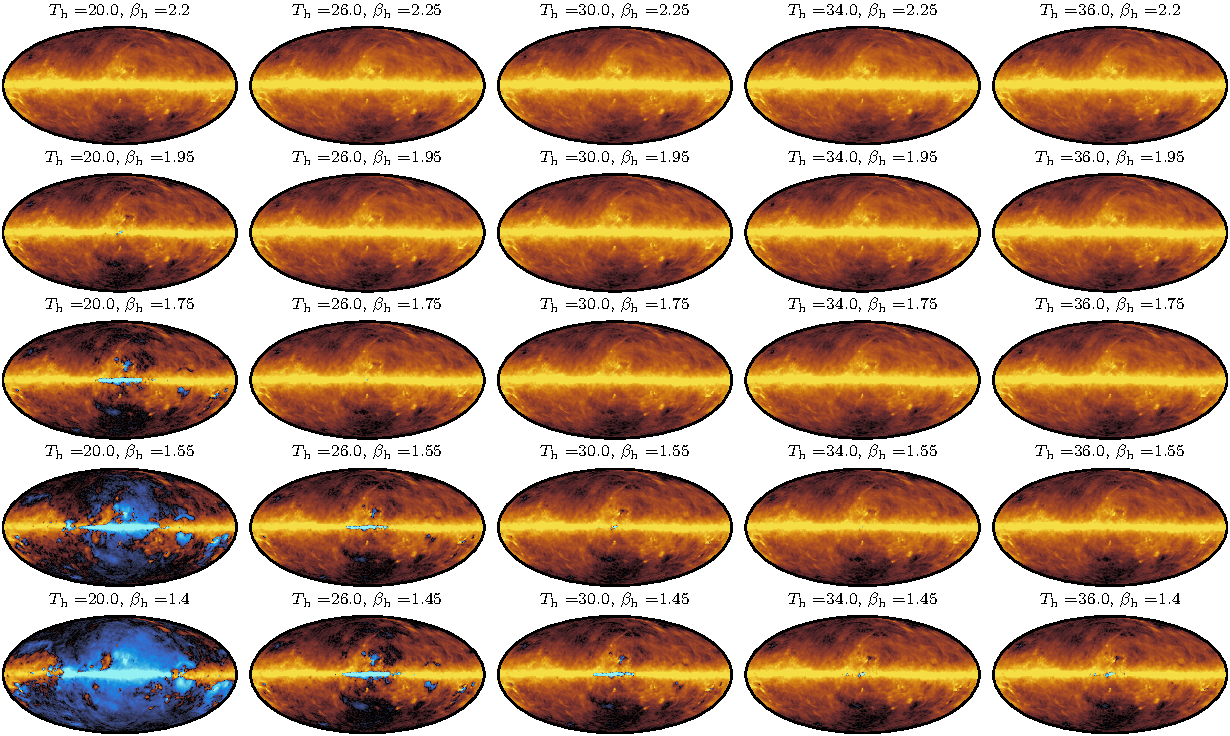
\includegraphics[width=\linewidth]{figures/HotDust_cold_Grid.pdf}
    \caption{Cold dust (\ion{H}{I} correlated dust) amplitudes for varying $T_\mathrm{h}$ and $\beta_\mathrm{h}$ values with all other grid parameters set to the fiducial values as recorded in \cref{tab:SEDs}. The central panel is the fiducial map. The corresponding hot dust maps can be seen in \cref{fig:hot_hot_dust_set}.}
    \label{fig:hot_cold_dust_set}
\end{figure*}

\subsection{Cold dust SED grid (\texorpdfstring{$T_{\mathrm{cold}}$}{T cold} and \texorpdfstring{$\beta_{\mathrm{cold}}$}{b cold})}
\label{sec:colddust}

\begin{enumerate}
    \item Add summary statistics plots from grid search
    \item Add/update full grid search plane 
\end{enumerate}

\begin{figure*}
    \centering
    \includegraphics[width=\linewidth]{figures/ColdDust_hot_Grid.pdf}
    \caption{Hot dust (\ion{C}{II} correlated dust) amplitudes for varying $T_\mathrm{c}$ and $\beta_\mathrm{c}$ values with all other grid parameters set to the fiducial values as recorded in \cref{tab:SEDs}. The center panel is the fiducial map. The corresponding cold dust maps can be seen in \cref{fig:cold_cold_dust_set}. }
    \label{fig:cold_hot_dust_set}
\end{figure*}

\begin{figure*}
    \centering
    \includegraphics[width=\linewidth]{figures/ColdDust_cold_Grid.pdf}
    \caption{Cold dust (\ion{H}{I} correlated dust) amplitudes for varying $T_\mathrm{c}$ and $\beta_\mathrm{c}$ values with all other grid parameters set to the fiducial values as recorded in \cref{tab:SEDs}. The central panel is the fiducial map. The corresponding hot dust maps can be seen in \cref{fig:cold_hot_dust_set}.}
    \label{fig:cold_cold_dust_set}
\end{figure*}

%  The cold dust component very neatly correlates strongy with the HI4PI data set, which maps the neutral hydrogen signature in the Milky Way. Since neutral hydrogen is only present in cold areas of the Milky Way, it is expected that these two should correlate spatially, though the HI4PI maps are not used as a template for this analysis. 

\begin{figure}
    \centering
    \includegraphics[width=\linewidth]{figures/dust_map.pdf}
    \caption{Cold dust}
    \label{fig:dust_cold}
\end{figure}

We compare the cold dust to the HI4PI maps using a standard pixel-by-pixel correlation,
\begin{align}
    \rho_{\mathrm{HI4PI,CD}}=\frac{1}{N-1}\sum_p^N\frac{(a_{\mathrm{CD},p}-\overline{a}_{\mathrm{CD}})(a_{\mathrm{HI4PI},p}-\overline{a}_{\mathrm{HI4PI}})}{\sigma_{\mathrm{CD}}\sigma_{\mathrm{HI4PI}}}
\end{align}
where $a_p$ are the pixel-by-pixel amplitudes in the two maps, and $\overline{a}$ are the average amplitudes across the whole maps, and $\sigma$ the map standard deviations. 
The cold dust resolution is reduced to \nside\ of 1024 with a beam of 16.2 arcmin to match the resolution of the HI4PI maps.
We find the two maps have a Pearson correlation coefficient of 0.93 (applying the same $\chi^2$ mask as in \cref{fig:chimask}). 





\subsection{Nearby dust SED grid (\texorpdfstring{$a_{\mathrm{near}}$}{a near}, \texorpdfstring{$T_{\mathrm{near}}$}{T near} and \texorpdfstring{$\beta_{\mathrm{near}}$}{b near})}
\label{sec:hotpah}

\begin{enumerate}
    \item Add TT-correlation plot between nearby and cold dust, and nearby and hot dust?
    \item Add summary statistics plots from grid search
    \item Add/update full grid search plane 
    \item Discuss the template a bit more maybe? Edenhofer...
\end{enumerate}

The nearby dust parameters (amplitude and spectral indices) are fixed to the \GAIA-based dust extinction template by \citet{edenhofer:2024}, which covers distances up to 1.25 kpc. This primarily uses \GAIA\ distances and extinction estimates to build a 3D map of the nearby dust from \citet{2023Zhang}, which also leverages the two micron all sky survey (2MASS), the wide-field infrared survey explorer (WISE and unWISE), the large sky area multi-object fibre spectroscopic telescope (LAMOST). We use the total integrated dust map for out model in this analysis. 

\begin{figure}
    \centering
    \includegraphics[width=\linewidth]{figures/hotPAH_map.pdf}
    \caption{Nearby dust. }
    \label{fig:dust_near}
\end{figure}

\subsection{\texorpdfstring{$\mathrm{H}_\alpha$}{Ha} correlated dust SED grid (\texorpdfstring{$a_{\mathrm{H}\alpha}$}{a Ha}, \texorpdfstring{$T_{\mathrm{H}\alpha}$}{T Ha} and \texorpdfstring{$\beta_{\mathrm{H}\alpha}$}{b Ha})}
\label{sec:halpha}


\begin{enumerate}
    \item Discuss poor control due to low signal, choice to use the results from DIRBE as fiducial
    \item Add summary statistics plots from grid search
    \item Add/update full grid search plane 
    \item Discuss the template a bit more maybe? WHAM and DIRBE results, why is this an extinction?
\end{enumerate}

% Why do we think H-alpha has extinction?
% The warm ionized medium is characterized by the \ion{H}{$\alpha$} signature, and in the case of the \Planck\ bands appears as an extinction term, likely due to the warm gas absorbing the light from hotter dust in the background. (??? why is it an extinction term)
\begin{figure}
    \centering
    \includegraphics[width=\linewidth]{figures/dust_Ha_map.pdf}
    \caption{Dust extinction. }
    \label{fig:extinction}
\end{figure}


\section{Efficiency assessment and goodness-of-fit}
\label{sec:gof}

\begin{enumerate}
    \item update efficiency plot
    \item discuss efficiency and residuals (appendix)
    \item 
\end{enumerate}


\begin{figure*}
    \centering
    \includegraphics[width=\linewidth]{figures/AvgDust_Grid_plotres.pdf}
    \caption{Left most column shows the sum of the dust maps averaged for each band (plus the residuals), and the middle column the corresponding residuals (with the same colourbar range). The final column shows the residuals with the colour bar scaled down by a factor of 100 so as to more easily see the structure in the residuals. The structure in the residuals indicates there may be still some zodiacle light, and that the CO lines, particularly in the 100~GHz bands could be improved. Additionally, it appears that the 545~GHz gain may also be able to be improved upon in future analysis. All the maps have been smoothed by 2 degrees for clarity.}
    \label{fig:MapsVsResiduals}
\end{figure*}


\begin{figure}
    \centering
    \includegraphics[width=\linewidth]{figures/All_efficiency.pdf}
    \caption{Efficiency of the dust model representing the data. Taking the input map minus the non-dust components (e.g. CMB, free-free, CO) squared minus the residuals sqaured, divided by the residuals squared and summed across the map we can measure how much of the signal is represented by the model and find that it is greater than 98\% across all HFI bands in blue. There is one point for each band, though many are overlapping. When we average the individual detector maps at each frequency (orange) we find that the final efficiency is greater than 99\% across all frequencies. This can also be seen clearly in \cref{fig:MapsVsResiduals} where it is clear that the residuals are around 100 times smaller than the dust signal at each band.}
    \label{fig:efficiency}
\end{figure}


\begin{figure*}
    \centering
    \includegraphics[width=\linewidth]{figures/dustFrac.pdf}
    \caption{Average dust from each component contributing to the total dust signal. }
    \label{fig:dustFrac}
\end{figure*}



\section{Correlations with external line emission maps}
\label{sec:correlations}
\begin{itemize}
    \item Add side by side plot of Hi4PI and cold dust? -> not this should come 
    \item Add TT-correlation plot between Hi4PI and cold dust, and Dame CO and cold dust?
    \item Discuss correlation coeff between Hi4Pi and cold dust (mention masks), maybe mention CO
\end{itemize}

% \begin{figure*}
%   \centering
%   \includegraphics[width=0.49\linewidth]{figures/CGDR2_colddust_1deg_n512_v1.pdf}
%   \includegraphics[width=0.49\linewidth]{figures/HI4PI_NHI_n0064_60arcmin_rescaled_TQU.pdf}\\
%   \includegraphics[width=0.49\linewidth]{figures/CGDR2_hotdust_1deg_n512_v1.pdf}
%   \includegraphics[width=0.49\linewidth]{figures/init_CII_firas_n16_v20.pdf}
%   \caption{Comparison of \Cosmoglobe\ DR2 thermal dust maps with respective line emission tracers.  }
%   \label{fig:dustmaps}
% \end{figure*}

\begin{figure*}
  \centering
  \includegraphics[width=\linewidth]{figures/dustComp}
  \caption{Comparison of \Cosmoglobe\ DR2 thermal dust maps with respective line emission tracers.  }
  \label{fig:dustmaps}
\end{figure*}


\begin{figure}
    \centering
    \includegraphics[width=\linewidth]{figures/correlation_plot.pdf}
    \caption{Correlation between dust components and tracers. The correlation between the hot dust and the CII emission seen in FIRAS, as well as the cold dust and the HI4PI HI emission are very strong.}
\end{figure}

\begin{figure}
    \centering
    \includegraphics[width=\linewidth]{figures/hot_cii_corr.pdf}
    \caption{Pixel-Pixel correlation between the hot dust and Firas CII maps. Both maps are at \nside\ 16 with a 420 arcminute beam.}
    \label{fig:hotCiiCorr}
\end{figure}

\begin{figure}
    \centering
    \includegraphics[width=\linewidth]{figures/cold_hi4pi_corr.pdf}
    \caption{Pixel-Pixel correlation between the cold dust and HI4PI maps. Both maps are at \nside\ 64 with a 16.2 arcminute beam.}
    \label{fig:coldHI4PICorr}
\end{figure}

\begin{figure}
    \centering
    \includegraphics[width=\linewidth]{figures/scatter_HI4PI_hot_totmask_n32.pdf}
    \caption{Theil-Sen fits to the hot dust, choosing three different HI4PI offsets ($2.0\times10^{20}$, $2.5\times10^{20}$ and $3.0\times10^{20}$).}
    \label{fig:hotHI4PIScatter}
\end{figure}

\begin{figure}
    \centering
    \includegraphics[width=\linewidth]{figures/scatter_HI4PI_cold_totmask_n32.pdf}
    \caption{Theil-Sen fits to the cold dust, choosing three different HI4PI offsets ($2.0\times10^{20}$, $2.5\times10^{20}$ and $3.0\times10^{20}$).}
    \label{fig:coldHI4PIScatter}
\end{figure}




\section{Modified blackbody fit to multi-component dust model}
\label{sec:mbb}

Commander1 on dust model




%\section{Future directions}
%\label{sec:future} 


\section{Conclusions}
\label{sec:conc}
% Using physically motivated dust models, we produce four new dust maps from the \planck\ PR4 HFI maps. These dust models include a cold dust component, a hot dust component (correlated with \ion{C}{II}), a nearby dust component (), and a dust extinction component (correlated with \ion{H}{$\alpha$}). These new models show improvement over previous \planck\ results, with ADD PHYSICAL REASON WE KNOW ITS BETTER. Previous analysis has indicated that a two-component dust model should out-preform the legacy single-component dust model, and this has further added physical tracers for the various components. Future analysis with the time-ordered HFI data will see further improvements to the HFI maps as well as the component separated maps, and we expect results from other experiments (CMB and beyond) to both benefit from, and contribute to, these new component maps. 

% In this analysis we only explore the intensity or dust temperature, future work should explore the polarized dust in a similar manner, with the aim of creating physically motivated dust templates as was done in Eiriks paper ADD REFERENCE. Future work will also explore the HFI data from the raw time-ordered data (as was done in \Cosmoglobe\ DR1 and \BeyondPlanck ADD REFERENCES) including the updated dust models here from the \npipe\ analysis. This will lead to improved gain modeling, and zodiacal light modeling, two obvious areas of improvement when considering the residuals (see \cref{app:residuals}). 
% These dust templates have been applied to the \Cosmoglobe\ DR2 results with DIRBE, and results can be seen in Eiriks second paper ADD REFERENCE. 
% We have already seen great benefit in using data sets beyond the standard CMB maps, and we expect with many high-fidelity experiments online or soon to come online (SUCH AS? SPHEREX? SO? ), we may find more or better tracers of the dust, allowing us to further improve these models. 

\begin{acknowledgements}
 Some of the results in this paper have been derived using the HEALPix \citep{HEALPIX} package.
  We acknowledge the use of the Legacy Archive for Microwave Background Data
  Analysis (LAMBDA), part of the High Energy Astrophysics Science Archive Center
  (HEASARC). HEASARC/LAMBDA is a service of the Astrophysics Science Division at
  the NASA Goddard Space Flight Center.  
\end{acknowledgements}


\bibliographystyle{aa}
% \bibliography{../../common/CG_bibliography,references,../../common/Planck_bib}
\bibliography{../../common/CG_bibliography,references,Planck_bib}


\appendix
\section{Residuals}
\label{app:residuals}
We can see the fidelity of the sky model by looking at the difference between the data and the model at each of the bands (see \cref{fig:residuals}). The residuals indicate potential for improvement to the modelling of the zodiacal light, as well as improvements to the 545~GHz gain. The incredibly low residuals in the 100, 143, 217 and 353~GHz maps demonstrate the great capabilities of this model. 

\begin{figure*}
    \centering
    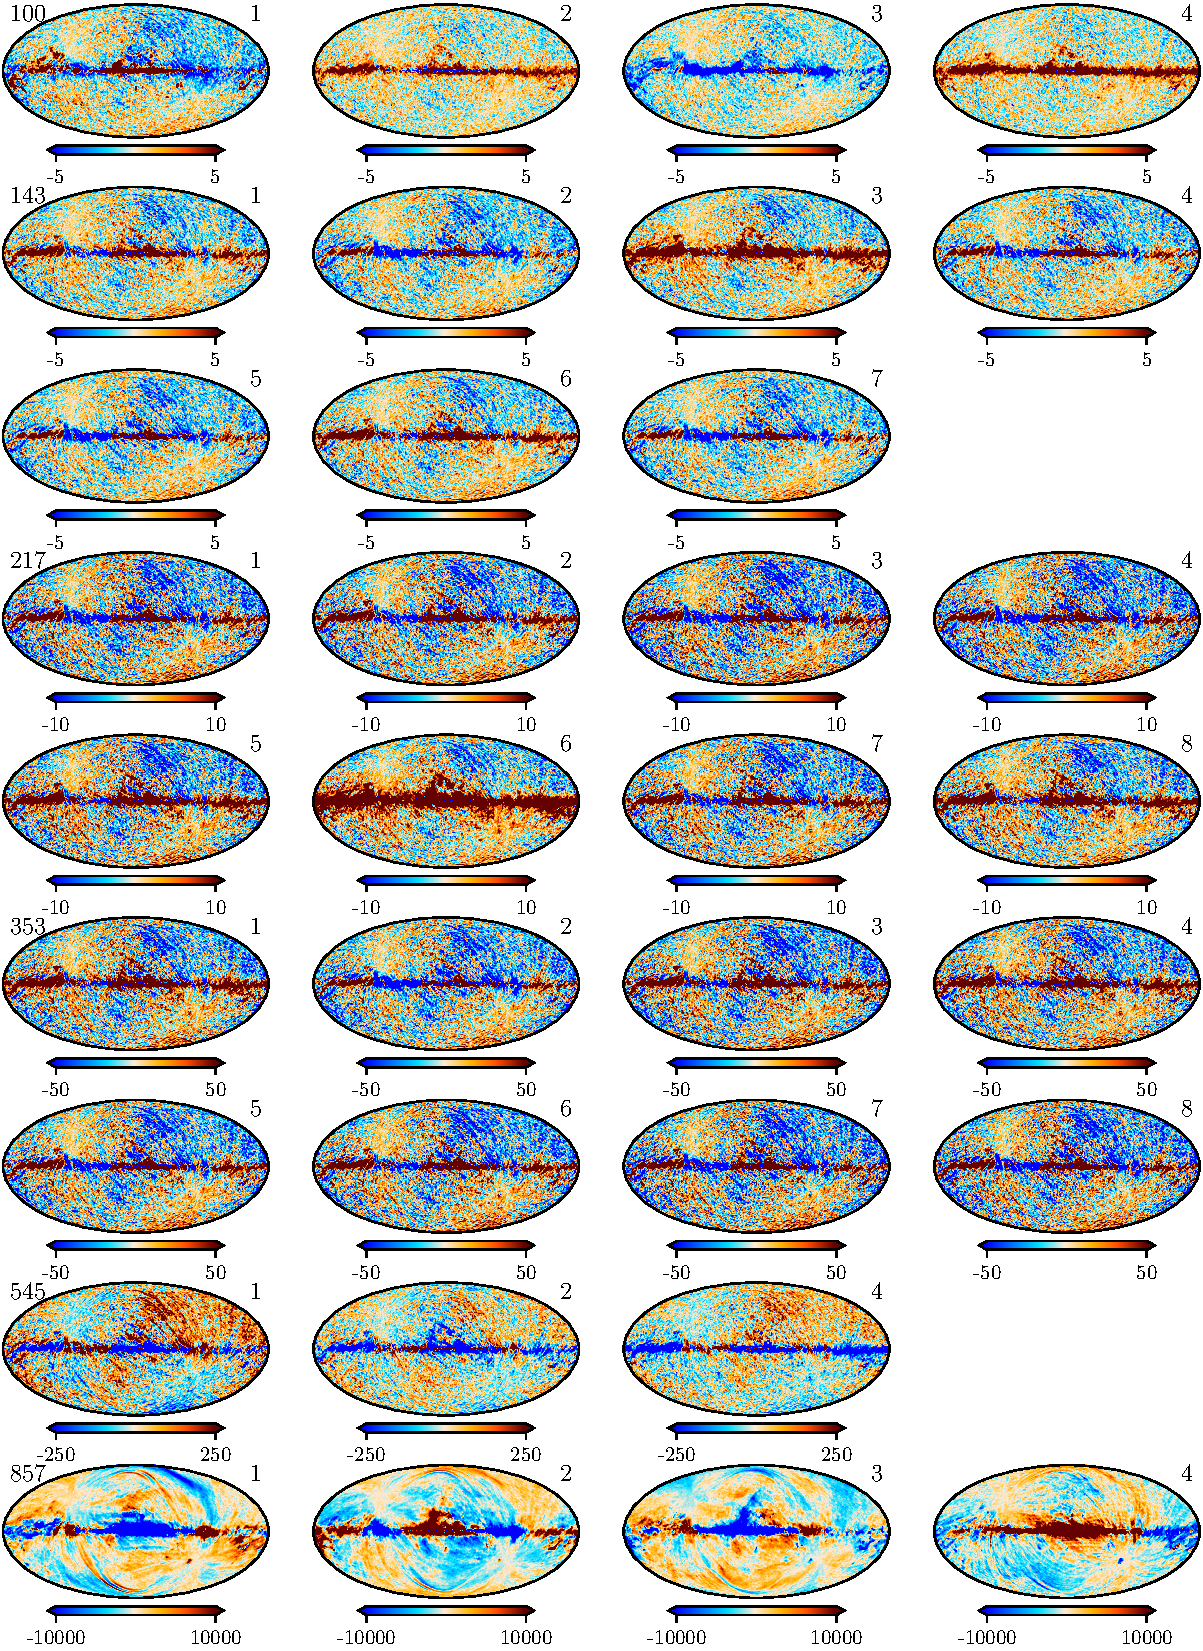
\includegraphics[width=\linewidth]{figures/residuals_plotres.pdf}
    \caption{Residuals (Data minus model) for the \planck\ HFI bands. Units are in $\mu K_\mathrm{CMB}$. The residuals hint at some uncorrected zodiacal light along the ecliptic plane, as well as potentially some improvements to the gain of the 545 channels.}
    \label{fig:residuals}
\end{figure*}


\section{Grid search tests}
\label{app:GridSearchTests}

\subsection{Cold dust}

\subsection{Nearby Dust}

\subsection{\texorpdfstring{H$\alpha$}{Ha} dust}

\end{document}
%%%% End of aa.dem


% \begin{figure}
%   \centering
%   \includegraphics[width=\columnwidth]{figures/chisq_353_alpha.pdf}
%   \caption{$\chi^2$ distribution for $\alpha$, the conversion factor from GAIA-based extinction to thermal dust emission at 545\,GHz, as evaluated from \Planck\ 353\,GHz data. The dashed vertical line indicates the best-fit value, and the dotted lines indicate the uncertainties. }
%   \label{fig:chisq_353_alpha}
% \end{figure}

% \begin{figure}
%   \centering
%   \includegraphics[width=\columnwidth]{figures/res_353-1_alpha097.pdf}\\
%   \includegraphics[width=\columnwidth]{figures/res_353-1_alpha099.pdf}\\
%   \includegraphics[width=\columnwidth]{figures/res_353-1_alpha101.pdf}
%   \caption{Residual maps at 353\,GHz as a function of $\alpha$. The middle panel corresponds to the best-fit value found in Fig.~\ref{fig:chisq_353_alpha}, while the upper and lower panels correspond to $\pm2\sigma$ deviations.}
%   \label{fig:res_353_alpha}
% \end{figure}


% \begin{figure}
%   \centering
%   \includegraphics[width=\columnwidth]{figures/res_100-1_1deg_v1.pdf}\\
%   \includegraphics[width=\columnwidth]{figures/res_143_1deg_v1.pdf}\\
%   \includegraphics[width=\columnwidth]{figures/res_217-1_1deg_v1.pdf}\\
%   \includegraphics[width=\columnwidth]{figures/res_545_1deg_v1.pdf}
%   \caption{Residual maps for each \Planck\ frequency channel that is included in the fit, evaluated for the best-fit scaling factor of $\alpha=625\,\mu\mathrm{K}_{\mathrm{CMB}}/\mathrm{ext}$. For the 100 and 217\,GHz channels, only the first horn maps are shown for brevity; the others appear visually similar.}
%   \label{fig:res_353_alpha}
% \end{figure}


% \begin{figure*}
%   \centering
%   \includegraphics[width=0.49\textwidth]{figures/dust_353-1_c0001_k000003.png}
%   \includegraphics[width=0.49\textwidth]{figures/ratio_353-1_dust_tot_2deg.png}\\
%   \includegraphics[width=0.49\textwidth]{figures/dust_cii_353-1_c0001_k000003.png}
%   \includegraphics[width=0.49\textwidth]{figures/ratio_353-1_dust_cii_tot_2deg.png}\\
%   \includegraphics[width=0.49\textwidth]{figures/hotPAH_353-1_c0001_k000003.png}
%   \includegraphics[width=0.49\textwidth]{figures/ratio_353-1_hotPAH_tot_2deg.png}
%   \caption{Comparison of the cold (\emph{top}), hot (\emph{middle}), and nearby (\emph{bottom}) thermal dust components as evaluated at 353\,GHz. The left column shows the absolute amplitude on a common linear color scale, while the right column shows the fraction of the given component relative to the sum of the three components. All maps are smoothed to an angular resolution of $2^{\circ}$ FWHM.   }
%   \label{fig:dust_353_ratio}
% \end{figure*}
